
%(BEGIN_QUESTION)
% Copyright 2007, Tony R. Kuphaldt, released under the Creative Commons Attribution License (v 1.0)
% This means you may do almost anything with this work of mine, so long as you give me proper credit

Configure a PID simulator for a {\bf temperature control} application.  Perform an open-loop test (stroking the control valve and examining the process variable response), and sketch the results:

$$\includegraphics[width=15.5cm]{i01742x01.eps}$$

Document some of the process characteristics observable in this test:

\vskip 20pt

Dead time ($L_R$ or $\tau_0$) = \underbar{\hskip 50pt} \hskip 50pt Lag time ($\tau$) = \underbar{\hskip 50pt} 

\vskip 10pt

Reaction rate ($R_R$) = \underbar{\hskip 50pt} \hskip 50pt Steady-state gain ($K$) = \underbar{\hskip 50pt}

\vskip 10pt

Process noise = \underbar{\hskip 70pt} \hskip 50pt {\it Self-regulating} or {\it integrating}?

\vskip 20pt

Estimate the values for P, I, and D you think will work well in this controller.  Qualitative answers such as ``aggressive,'' ``moderate,'' ``minimal,'' and ``none'' are okay to specify here!

\vskip 10pt

P = \underbar{\hskip 50pt} \hskip 50pt I = \underbar{\hskip 50pt} \hskip 50pt D = \underbar{\hskip 50pt}

\vskip 20pt

Next, tune the controller in closed-loop (automatic) mode, optimizing the P, I, and D parameters for rapid response to setpoint and load changes.  Some process oscillation is permissible, but no more than ``quarter-wave'' damping.  Document your final P, I, and D settings here:

\vskip 10pt

P = \underbar{\hskip 50pt} \hskip 50pt I = \underbar{\hskip 50pt} \hskip 50pt D = \underbar{\hskip 50pt}

\vskip 20pt

After this, with the controller still in closed-loop (automatic) mode, optimize the P, I, and D parameters for the most rapid response to setpoint and load changes {\it without any overshoot}.  Document your final P, I, and D settings here:

\vskip 10pt

P = \underbar{\hskip 50pt} \hskip 50pt I = \underbar{\hskip 50pt} \hskip 50pt D = \underbar{\hskip 50pt}

\vskip 10pt

\underbar{file i01742}
%(END_QUESTION)





%(BEGIN_ANSWER)

The ``answers'' can only be found by actually tuning a controller!  It is recommended to review the results of your tuning with your instructor to grasp the significance of each process and its PID tuning requirements.

%(END_ANSWER)





%(BEGIN_NOTES)


%INDEX% Control, PID tuning: computer simulation exercise (temperature control)

%(END_NOTES)


